% !TEX root = ../report.tex
\chapter{PCB}\label{chapter:pcb}

While the main objective of the project is to create a MIMD system, which essentially can be completed by FPGA design alone, everything depends on the PCB to complete the system. It is the final step in realizing the system as a whole, going from a theoretical dimension of design and ideas, to a physical one with components and electricity.

This chapter will attempt to explain in detail each step during the design process of the circuit board. The sections have been ordered as much as possible according to which stage in the process they occurred, with schematic drawings as the first step, choice of components as the second, followed by layout, and finally the test plan. While we have tried to divide these steps to our best ability, some of them are intertwined, like schematics and components, as you need of course to decide on what components your card will have before actually drawing them, unless you have a particular fondness for doing unnecessary work.

% !TEX root = ../../report.tex

\chapter{Schematics}\label{apx:schematics}

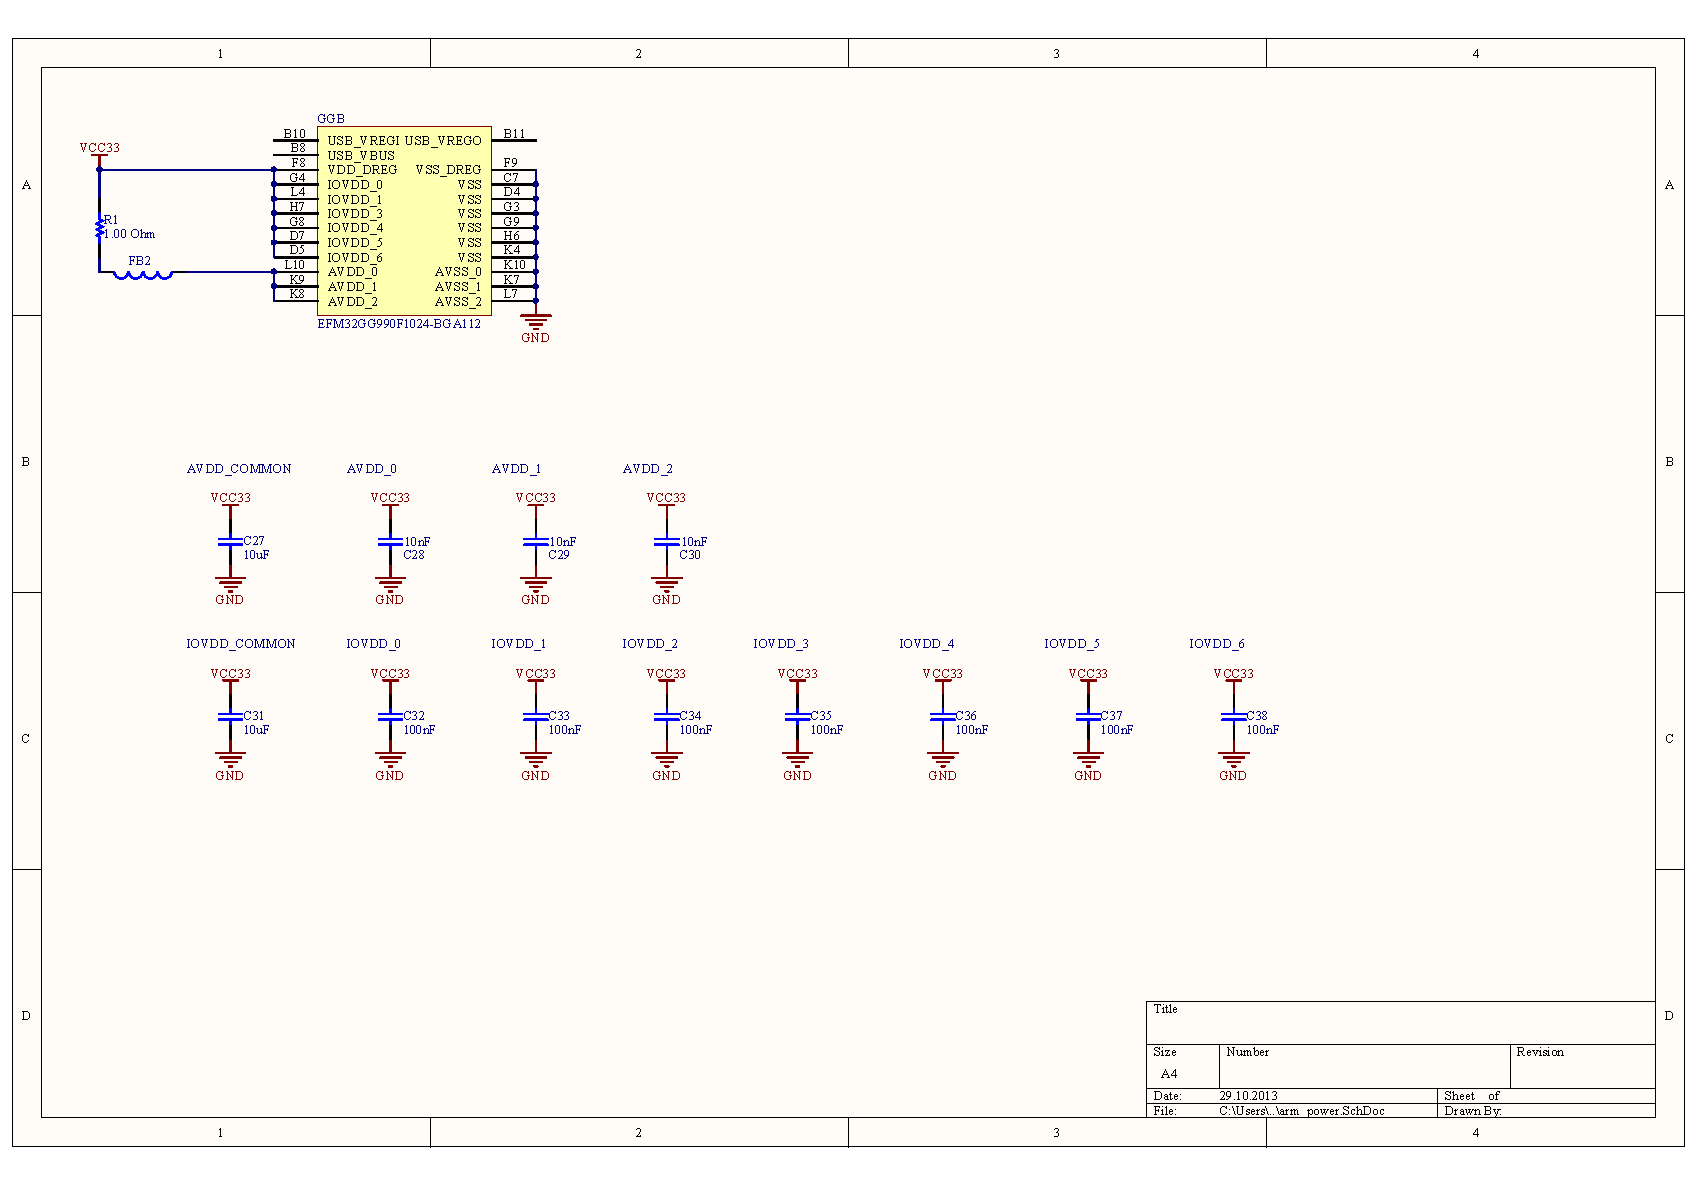
\includepdf[pages=-]{../pcb/take1/take1.pdf}
% !TEX root = ../../report.tex
\section{Components}

The PCB group was eager to learn how modern PCB production is done, using the
same tools and technologies as the industry. Thus, our choice of components was
strongly driven by a smaller is better mindset. The use of BGA packages (for
the MCU and FPGA) was already given from the resources we had available and the
fact that Odd Rune Lykkebo had experience baking these.

We used 0805 surface-mount components as much as possible, because they were the
smallest packages we could comfortably solder. This not only lowered the
production cost, but also allowed us to place components on both sides of the
board, and consequently minimizing the size.

{\bf USB-UART}
\begin{itemize}
  \item FTDI FT232RL - USB-UART converter
  \item 1x 4k7 and 1x 10k
  \item 3x 100nF and 1x 4.7uF
  \item USB3140-30-0170-1-C USB Micro B connector 
\end{itemize}


  



	

\section{Layout}
% !TEX root = ../../../../report.tex

\subsubsection{Routing}

Almost everything was autorouted, with only a few exceptions. The power supply had to be done manually, as well as the fanout on the FPGA. The routes are visible in the last image of Appendix~\ref{apx:schematics}.
% !TEX root = ../../report.tex
\section{Layer Stack}

We had three primary voltage levels on the PCB -- 1.2V, 1.8V and 3.3V. To
minimize resistance in the power distribution system, we decided to dedicate a
layer on the PCB to be used as a shared power plane. Another plane was used for
common ground and covered the whole PCB (excluding non-grounded through-holes).
This is setup with a shared ground and split power plane is common practice for
modern PCB design.

As for the signal layers, the BGA packages we used had only 0.8 mm pitch between
its feets. This forced us to have more signal layers than we originally set out
for, to be able to fanout and escape the BGA packages. Using a QFP-like package
could probably have saved us some cost, but using BGA gave us a valuable
experience on modern PCB design.

We settled upon a total of 8 layers on the PCB.

% !TEX root = ../../../../report.tex
\subsubsection{Footprints}

Each component is associated with a schematic drawing and a footprint. Because certain components were not available in public libraries they had to be drawn from scratch. Below is a list of all custom drawings and footprints.

\begin{table}[h]
	\centering
	\begin{tabular}{|l l l|}
		\hline
		\textbf{Component} & \textbf{Footprint}  & \textbf{Schematic} \\
		\hline
		XP Power Switch-Mode Regulator & X & X \\
		Würth Electronics MicroSD & X & X \\
		Molex MicroUSB AB & X & X \\
		Lumberg 3.5mm audio jack & X & X \\
		Buttons & X & X \\
		DC-10B & X & X \\
		Texas Instruments Op amp & X & X \\
		Diodes INC. Linear regulator& X & X \\
		Cypress Semiconductor SRAM & X & X \\
		& X & X \\
		& X & X \\
		& X & X \\
		& X & X \\
		\hline
	\end{tabular}
	\caption{Custom footprints and schematics}
	\label{tab:footprints}
\end{table}

\todo{finish table}

% !TEX root = ../../report.tex
\section{Test plan}

In order to ease the process of assembly after receiving the final PCB from 
production, we set up a test plan detailing step by step what we are planning
to do. The main idea of the plan is to catch potential errors in the PCB design
as early as possible so that if, and when, we run into a problem we can rule
out as many sources as possible.

\begin{enumerate}
    \item Manually test important solder points using a multimeter. This includes connections between the power source and regulators, as well as the connections from oscillators and clock generators to their source pins on the microcontroller and the FPGA. After checking these points we can assume that the components will boot correctly.
    \item After soldering the power supply we will need to check the provided voltage levels. This is an important point as sensitive components might be damaged if these are wrong. We are able to do this safely even after the major components are soldered as we have added headers allowing us to disconnect the power planes from the regulators. \todo{Is this last statement correct?}
    \item  \todo[inline]{We should investigate JTag boundary scan as suggested by Gunnar}
    \item After soldering the major components as well as the JTAG interfaces we should attempt to flash test programs. These programs will be provided by the FPGA and Software groups and will test both the respective component, the GPIO, as well as the interconnection between the two.
    \item After soldering the entire board we are going to test the more advanced user interfaces. This includes the UART over USB, and also the audio input and output. Testing this will be done by a specially prepared program from the Software group.
    \item Finally, after the FPGA and Software group have completed their work, or at least completed the design necessary to run any testing, we need to start measuring the overall power usage of the board. Using these measurements we will evaluate and possibly attempting to power our board using the 5V USB connection, as mentioned in section~\ref{psu:usb} - Power by USB.
\end{enumerate}

